\section{Clustering}
\label{sec:clustering}

One of the major limitations in building linear models is effective modeling of higher-order and cross-term interactions.  In order to generally survey these types of interactions, we built a basic clustering model in order to provide a superficial evaluation of cross-term interactions within the surveyed data.

\subsection{Algorithms}

Our clustering algorithm essentially made use of k-means clustering to produce a series of cluster centers representative of the data, and assign each point to one of the clusters.  Prediction was done by determining the mean distance to each cluster center (measured as the sum of the value differences between the new data and the cluster center), and assigning that data to the closest cluster center, which in turn was used to predict the most likely response based on the new data.

As before, the constant algorithm is extremely important in analysis of the models, and providing a lowere bound on classification performance.  Further comparisons were done between the results of clustering-based prediction using varied numbers of clusters.  The cluster counts selected were 2 (partitioning the data into ``drinker'' and ``non-drinker'' data), 6 (partitioning the data into a number of clusters equal to the number of possible responses), 10 (slightly more than the number of responses to allow for the fact that some clusters may round to the same response), and 20 (significantly more than the number of responses).

\begin{figure}[t]
\centering
\makebox[\textwidth][c]{
\subfigure[]{
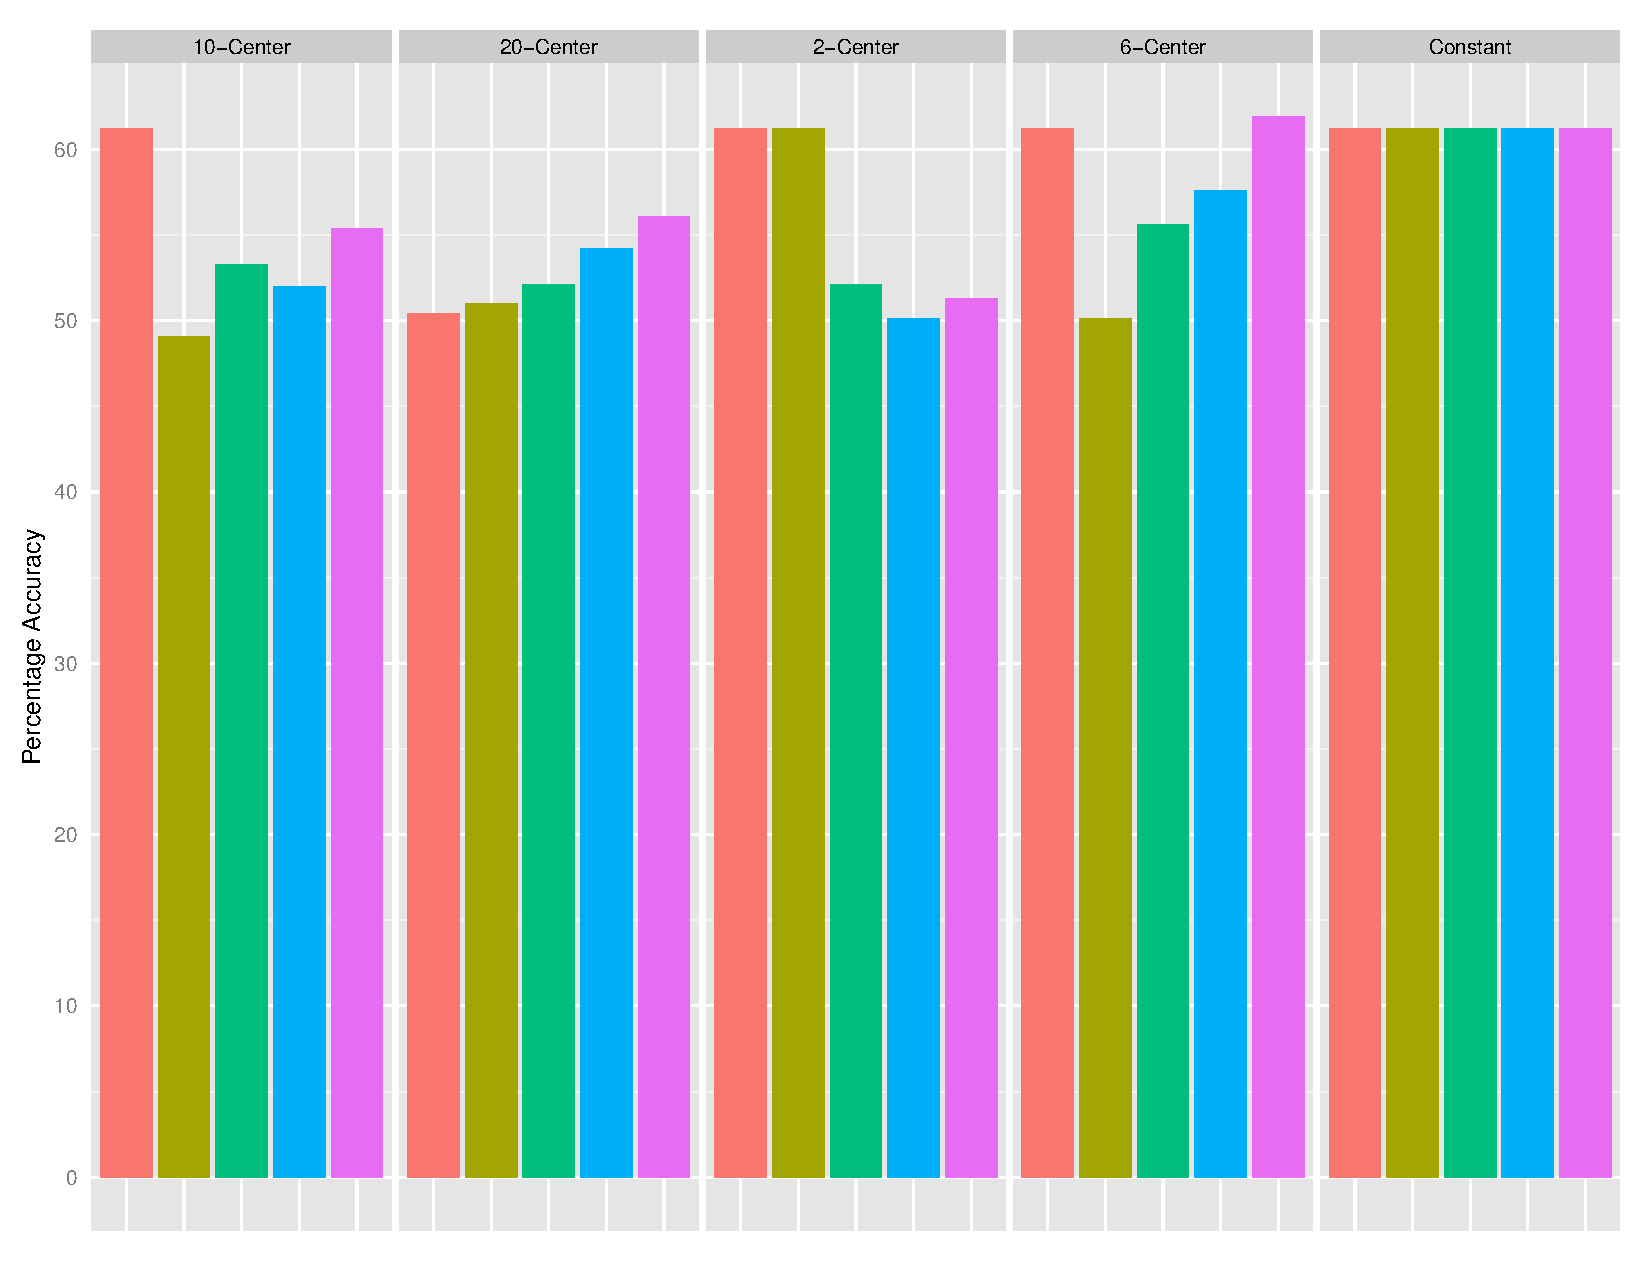
\includegraphics[scale=0.65]{clustering_percent.pdf}
\label{clustering_percent}
}
\subfigure[]{
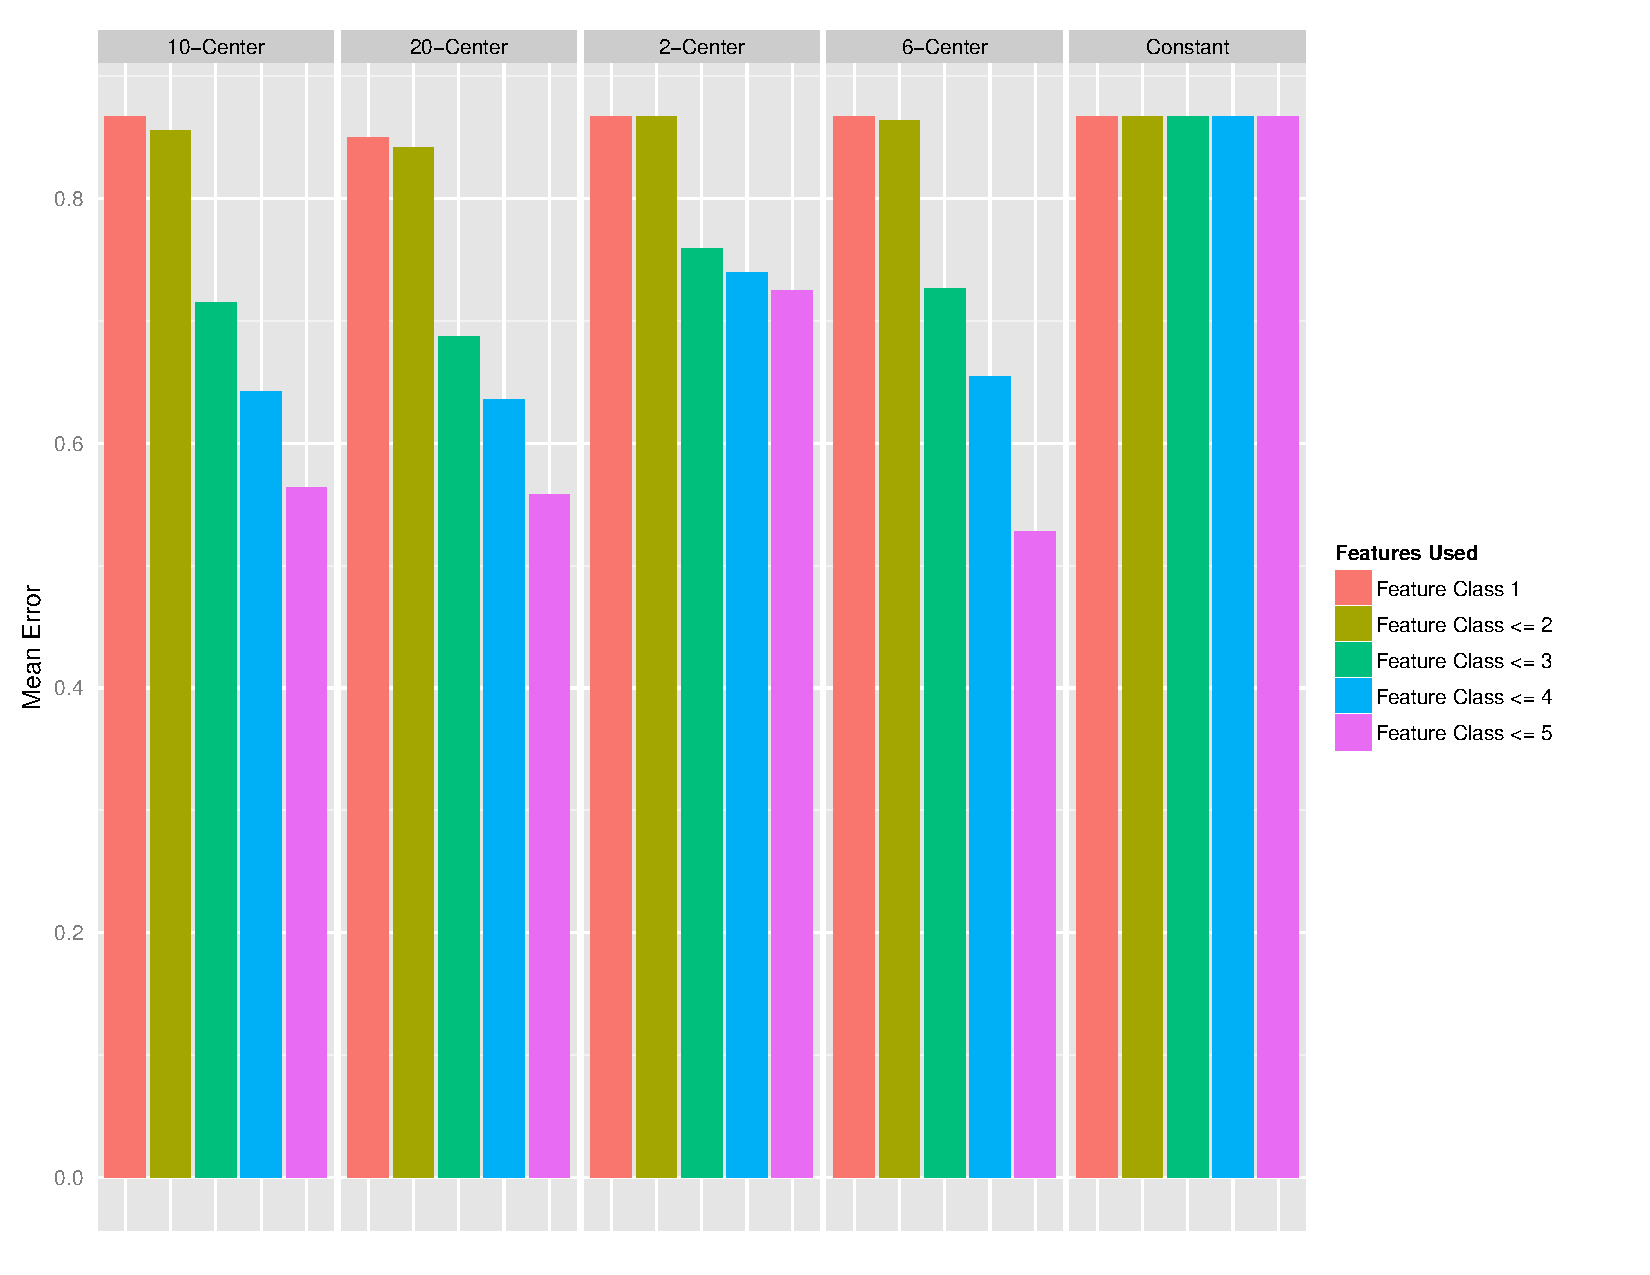
\includegraphics[scale=0.65]{clustering_error.pdf}
\label{clustering_error}
}
}
\caption{Predictive accuracy and mean error of the clustering algorithm over different cluster counts.}
\label{clustering_results}
\end{figure}

\subsection{Results}

Figure \ref{clustering_results} summarizes the performance of the clustering algorithm at the 4 chosen cluster counts using 5-fold cross validation on our training/testing dataset.  The constant algorithm is once again provided for reference.  Figure \ref{clustering_results} \subref{clustering_percent} shows the percent accuracy metric and Figure \ref{clustering_results} \subref{clustering_error} shows the mean error.  Overall the predictive capability of the clustering-based model was, as expected, quite limited.  On the whole, the model was only significantly able to outperform the constant algorithm when several of the higher feature classes were included. For only feature classes 1 and 2, the improvement was negligible.

As expected, an increased number of clusters offers improved performance. Particularly 2 clusters provides fairly poor ``predictive'' power, as predicting the response to a 6-answer question in only 2 classes is somewhat impractical. It is of note, however, that as the number of included feature classes increased, the improvement between the latter three cluster counts becomes negligible. Indeed, by the time all 5 feature classes are included, the results from those 3 are hard to distinguish.

\subsection{Extensions}

As the k-means clustering model is meant as a classification model, and not one with real predictive capacity, the means for extension here are somewhat limited. It is much more productive to preserve this methodology simply as an initial survey of the data, and use it to drive the analysis of more appropriate models as seen below. However, if we really did wish to employ this methodology toward prediction, there are a few salient adjustments we could make. For one, we could adjust the weight of various variables within the clustering to be able to more accurately fine-tune how the clusters are produced. This is unfortunately not possible within the tools available, and there is an unfortunate tradeoff between the number of variables we can introduce, and the amount of control we have over the influence of each variable on the entire sample. Another approach would be to consider additional schemes for interpreting cluster assignments. This is unfortunately where the limitations of the clustering approach begin to show themselves--because k-means clustering is not explicitly designed as a model with extremely effective predictive capacity, predicting responses simply by assigning points to their nearest cluster may not produce the desired result.
